\documentclass[notitlepage]{report}

\usepackage[a4paper,margin=0.5in]{geometry}
\usepackage{array}
\usepackage{xcolor}
\usepackage{graphicx}
\usepackage{float}
\usepackage{adjustbox}

\author{Niko Hellgren, 505174}
\title{Data Analysis and Knowledge Discovery, Assignment 2}
\linespread{1.14}
\renewcommand{\thesection}{\arabic{section}}

\begin{document}
\maketitle

\section{\textit{k}-NN prediction}
The model used was programmed in Python with little to no use of external libraries. The data was z-score standardized, pre-calculated into a sample distance matrix, which was then used to leave-one-out cross-validate the data. The CV-data was used to tune the value of $k$ to minimize the mean-square error (MSE) in the data. Since the classification is into discrete categories, the distance from the data point to the range that rounds to the correct value was considered in the calculation.

The results of the tuning process of $k$ is presented in Figure \ref{tbl:nn-mses}. Based on the results, the value $k=12$ gives the lowest error, albeit with little margin to the other low values. The cross-validation results of 12-NN are presented in Figures \ref{tbl:nn-scatter} and \ref{tbl:nn-conf}.

Despite the relatively low value of MSE, the results are not too good. The uneven distribution of samples in different qualities causes most samples to be predicted to be of quality 6, which makes up 44.9\% of the whole data set, with the range 5--7 making up 77.9\%. The low correlation between the features and the quality (as was seen in assignment 1) causes the evenly distributed 6-samples in the train set to pull most test samples to that class.

\begin{figure}[H]
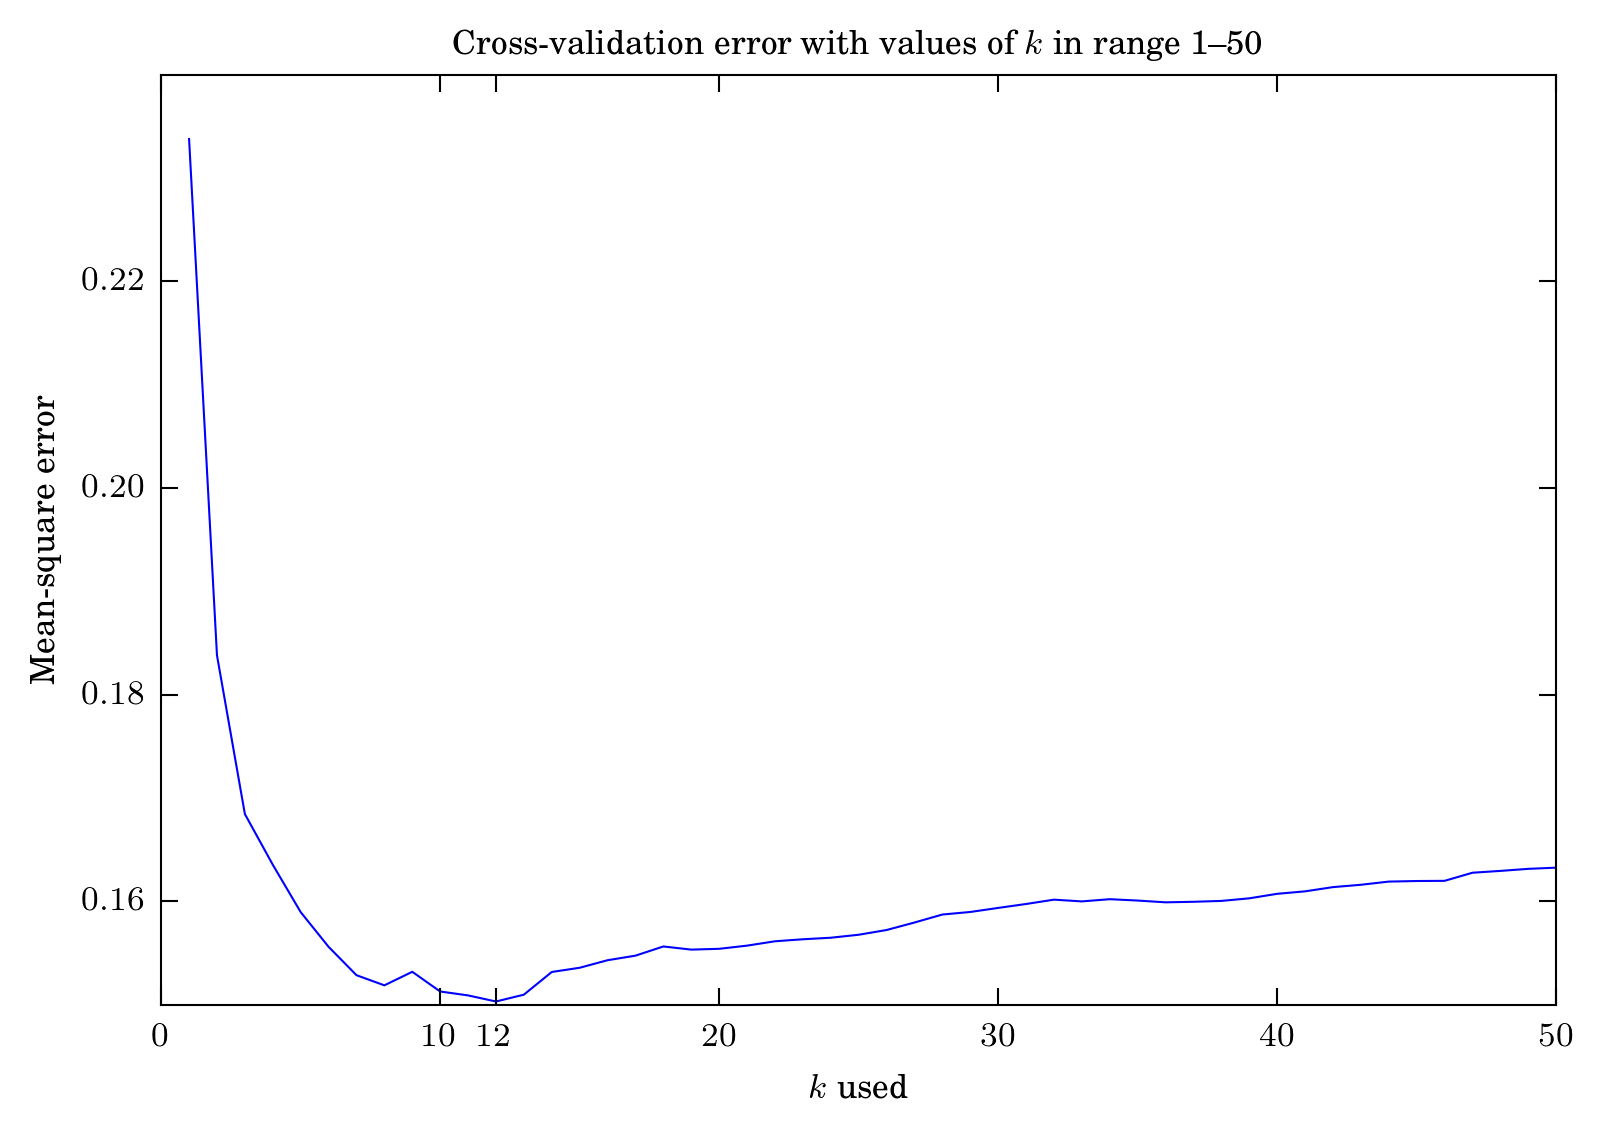
\includegraphics[width=\textwidth]{mse2_k1-50.png}
\caption{Errors of $k$-NN cross-validation}
\label{tbl:nn-mses}
\end{figure}

\begin{figure}
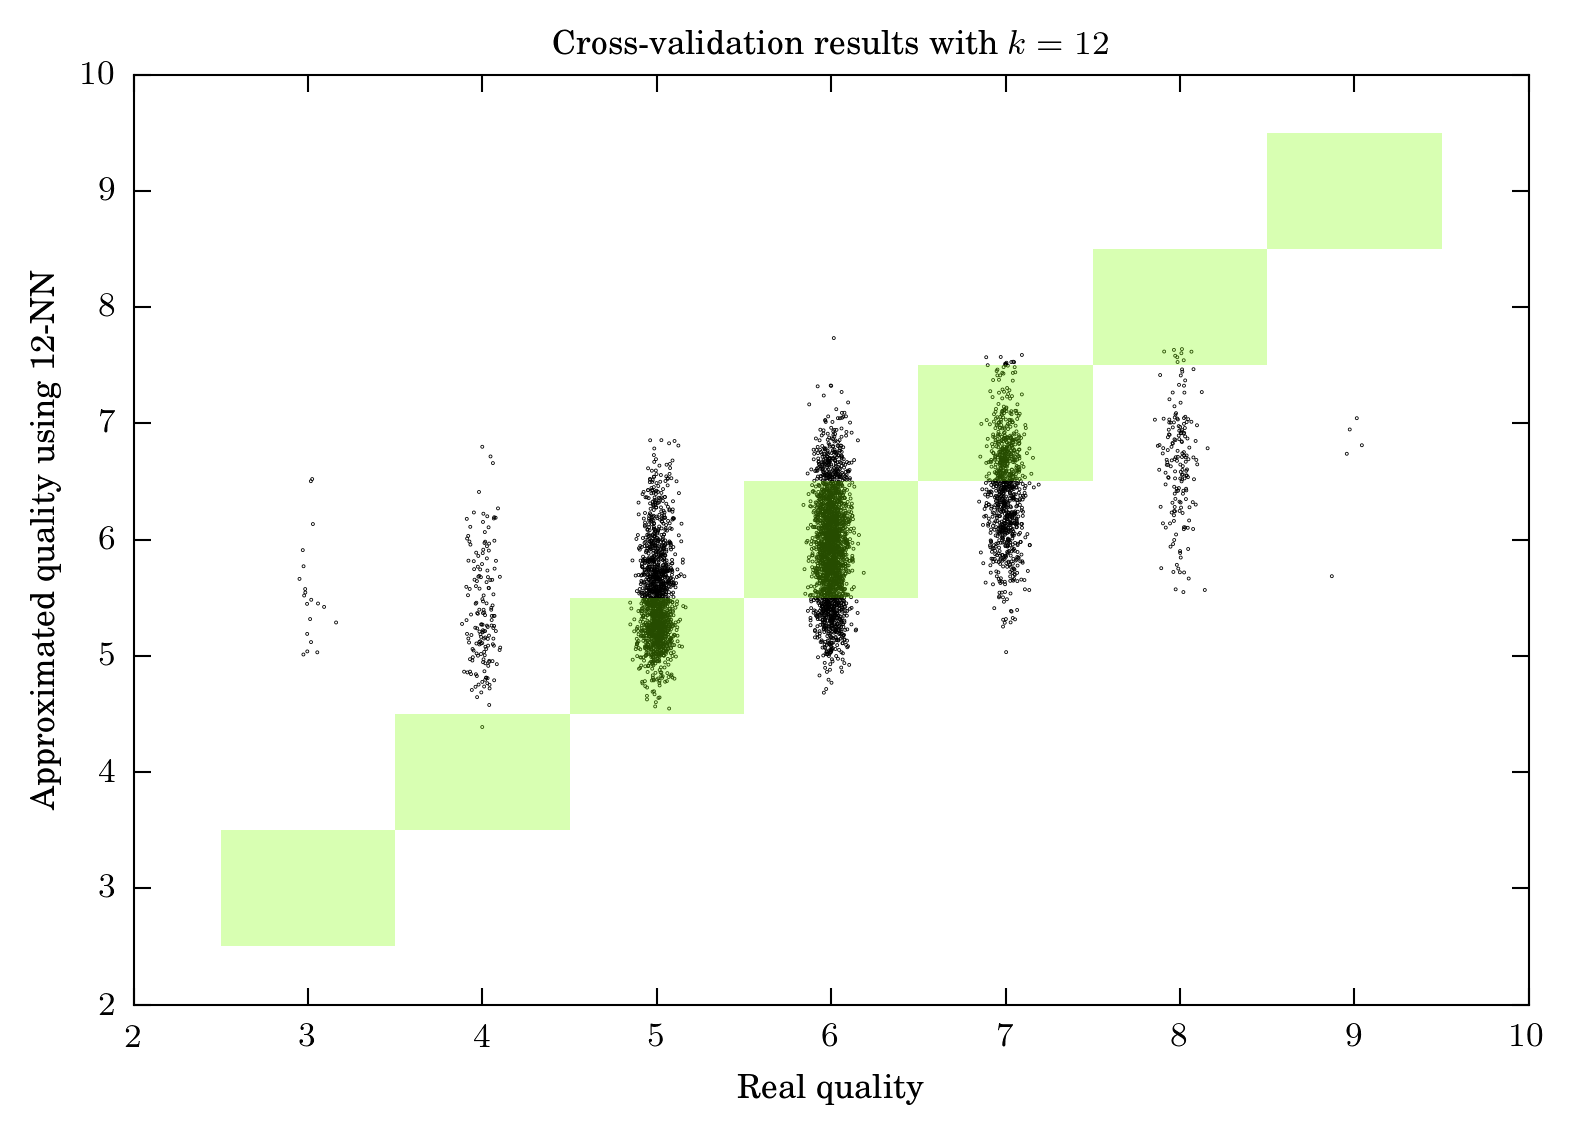
\includegraphics[width=\textwidth]{cv_scatters/12.png}
\caption{Results of 12-NN cross-validation as a scatter plot. The green boxes represent areas where the prediction is correct. All points have jitter following N(0,0.05) to avoid overlapping.}
\label{tbl:nn-scatter}
\end{figure}

\begin{figure}
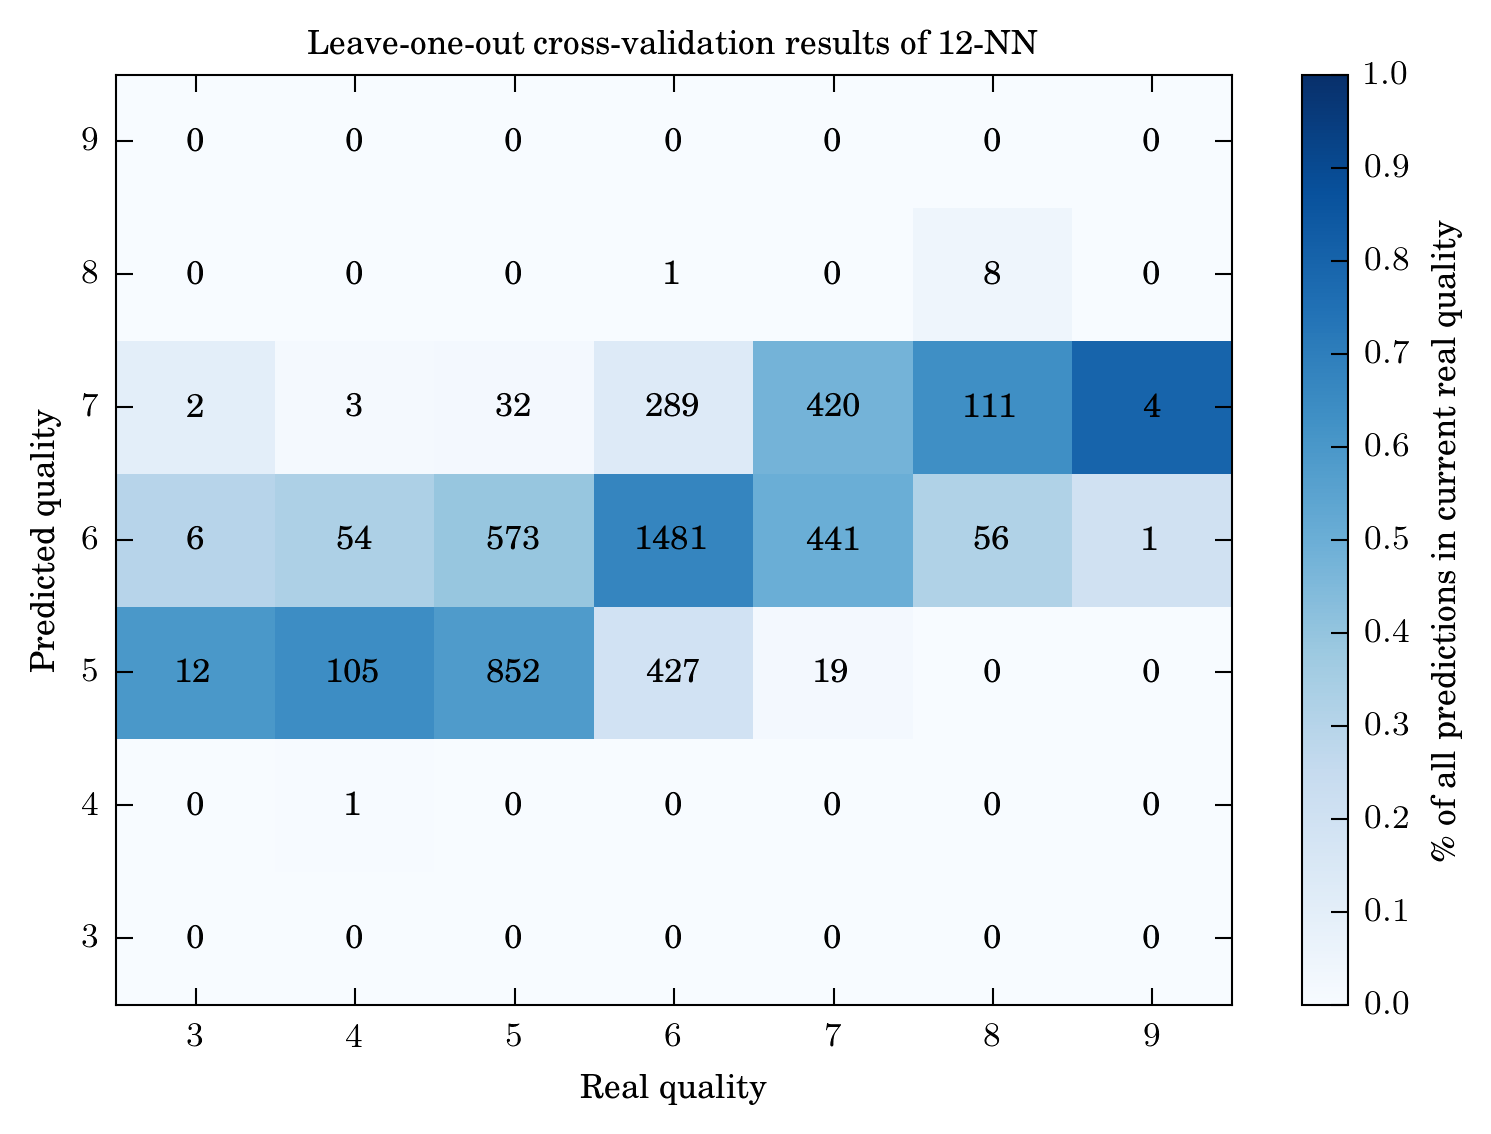
\includegraphics[width=\textwidth]{12-nn-cv.png}
\caption{Confusion matrix of 12-NN cross-validation}
\label{tbl:nn-conf}
\end{figure}
\newpage
\section{Linear regression}
Regression model was built using the examples presented in the lectures for Ridge regression. The same standardized data was used and leave-one-out cross-validated to determine a good value for the hyperparameter $\lambda$.

The results of the tuning process of $\lambda$ are presented in Figures \ref{tbl:reg-mses-15} and \ref{tbl:reg-mses}. Due to the random ordering of the samples, the values of $\lambda$ with the smallest error varied between runs, but was often the smallest with values around 40. The cross-validation results of Ridge regression with $\lambda=40$ are presented in Figures \ref{tbl:reg-scatter} and \ref{tbl:reg-conf}.

The MSE values are larger than with k-NN, and it can be seen as worse predictions. The samples in class 6 were very well predicted, but this is partially caused by the model predicting most of the test samples as quality 6.

\begin{figure}[H]
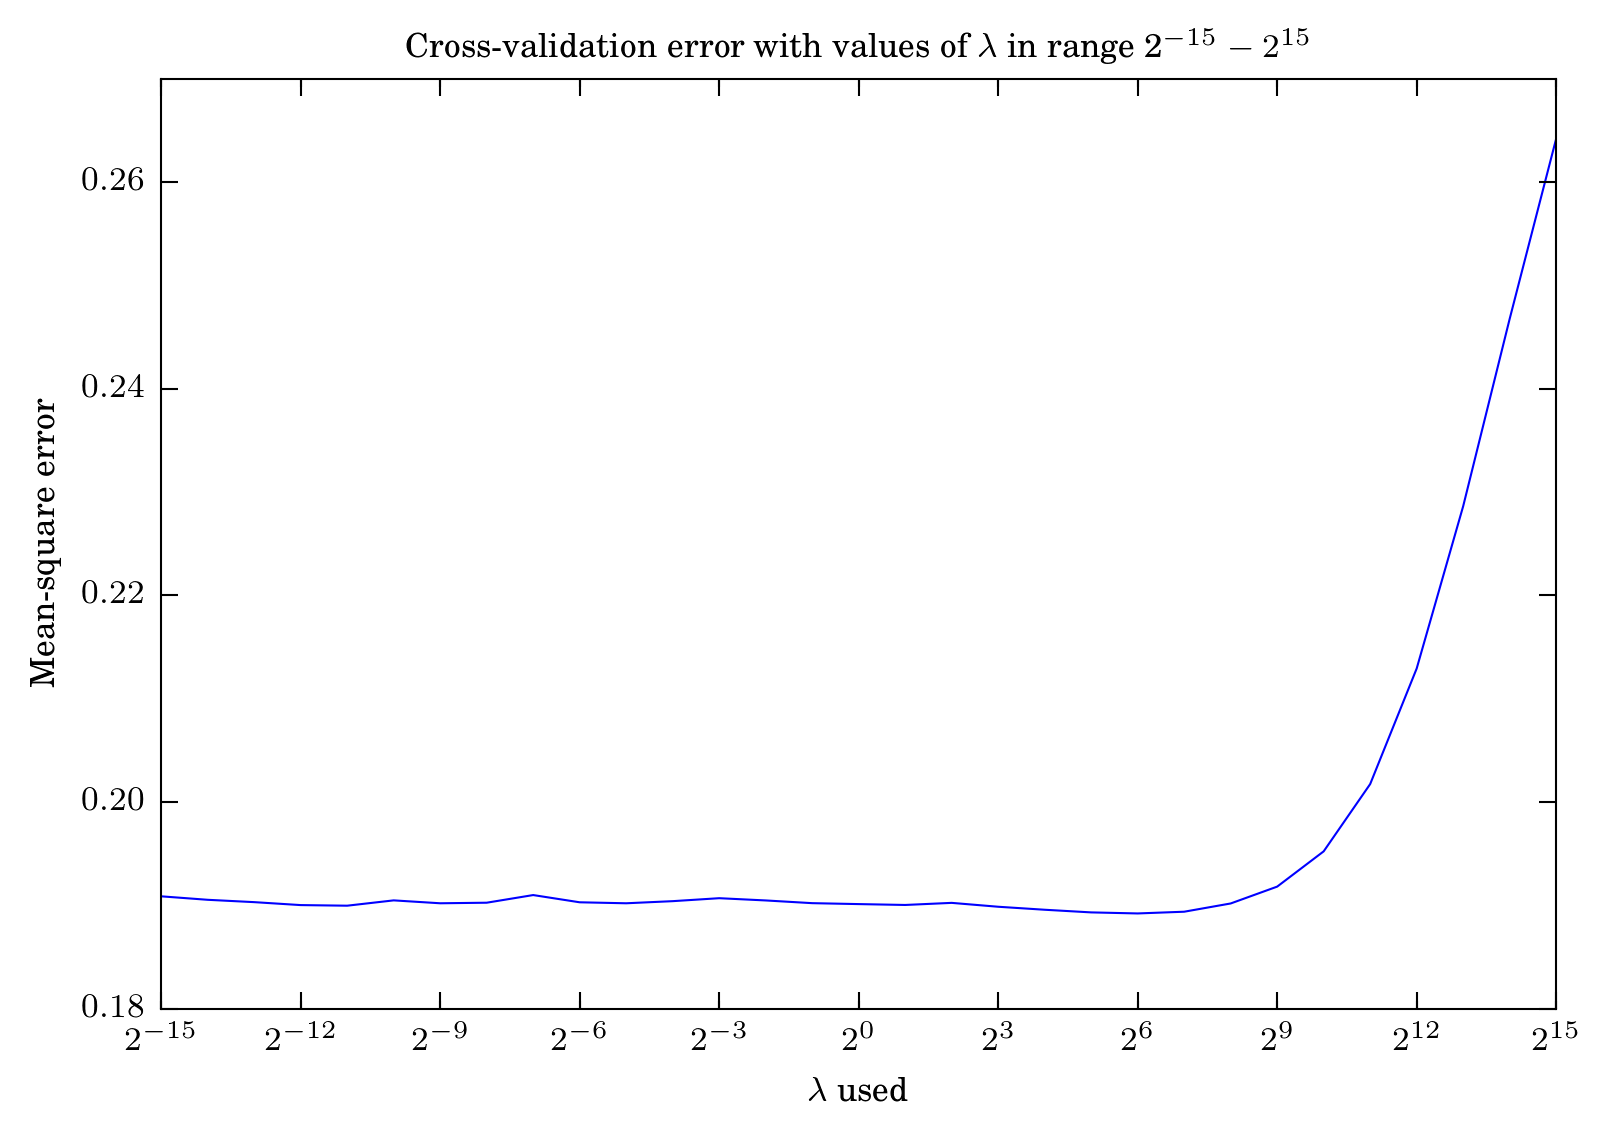
\includegraphics[width=\textwidth]{mse_lmbd15.png}
\caption{Errors of Ridge regression cross-validation}
\label{tbl:reg-mses-15}
\end{figure}

\begin{figure}[H]
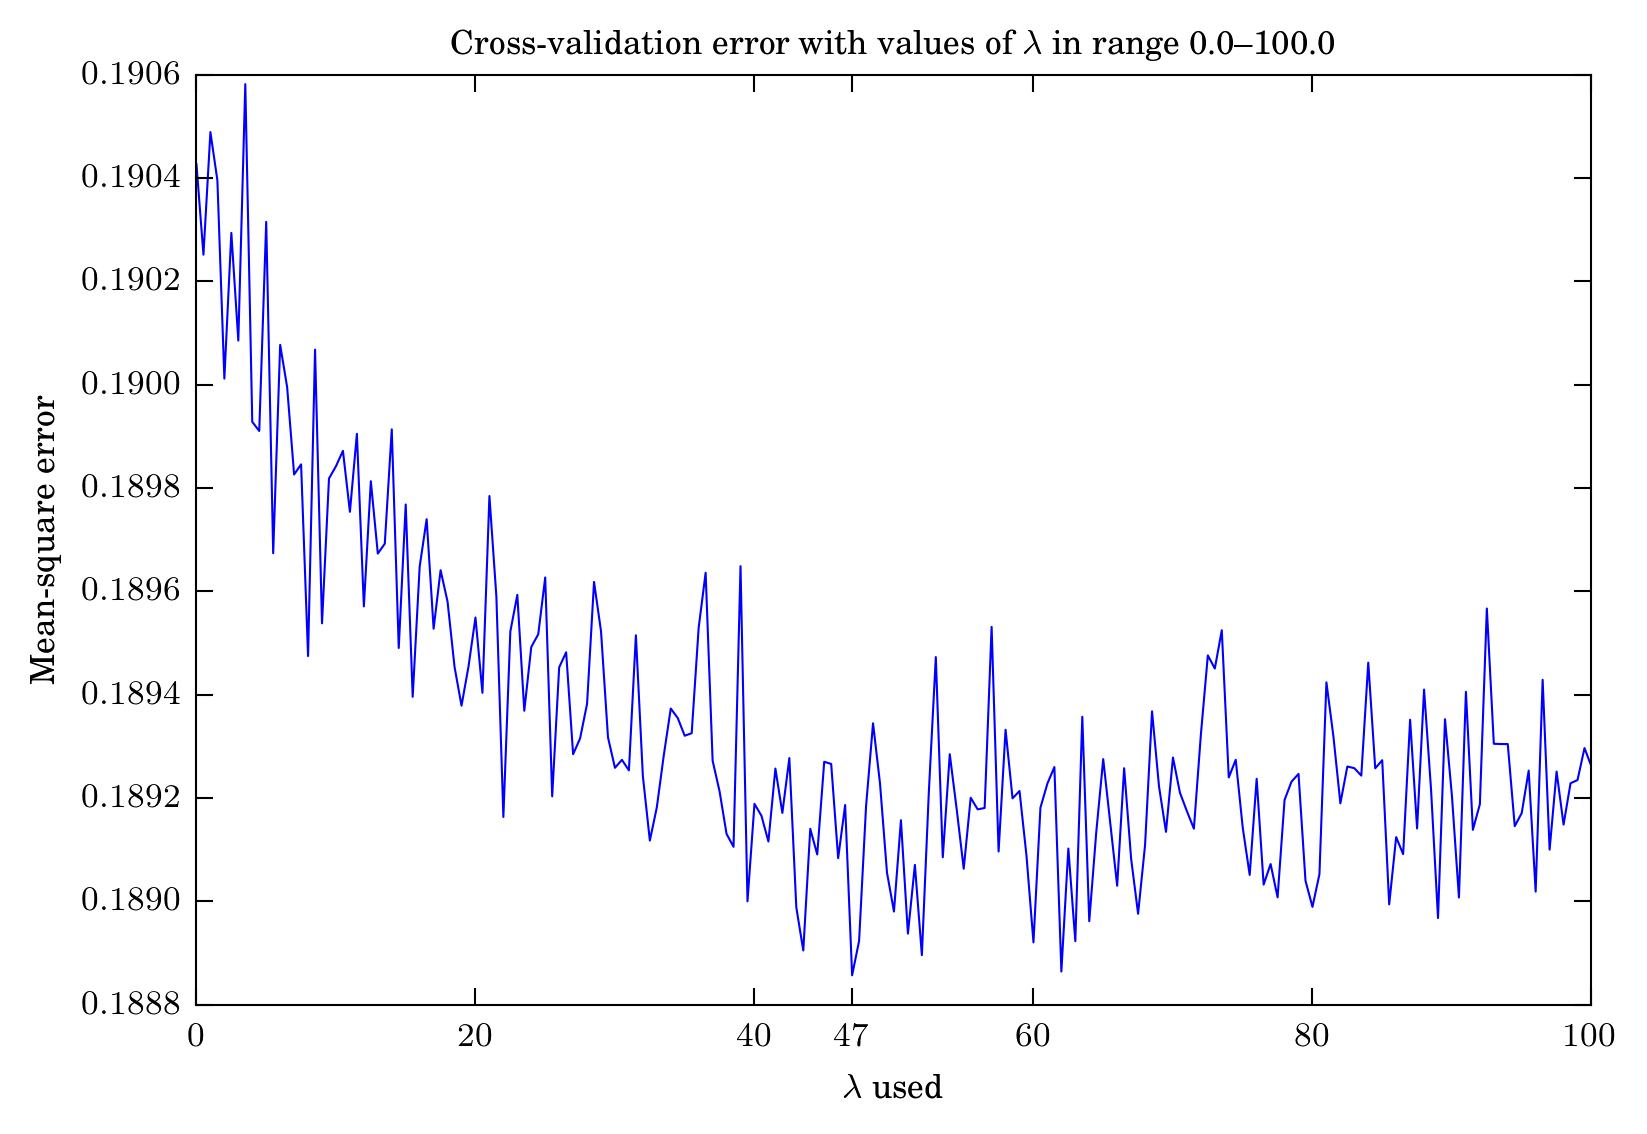
\includegraphics[width=\textwidth]{mse_lmbd.png}
\caption{Errors of Ridge regression cross-validation in a smaller range}
\label{tbl:reg-mses}
\end{figure}

\begin{figure}
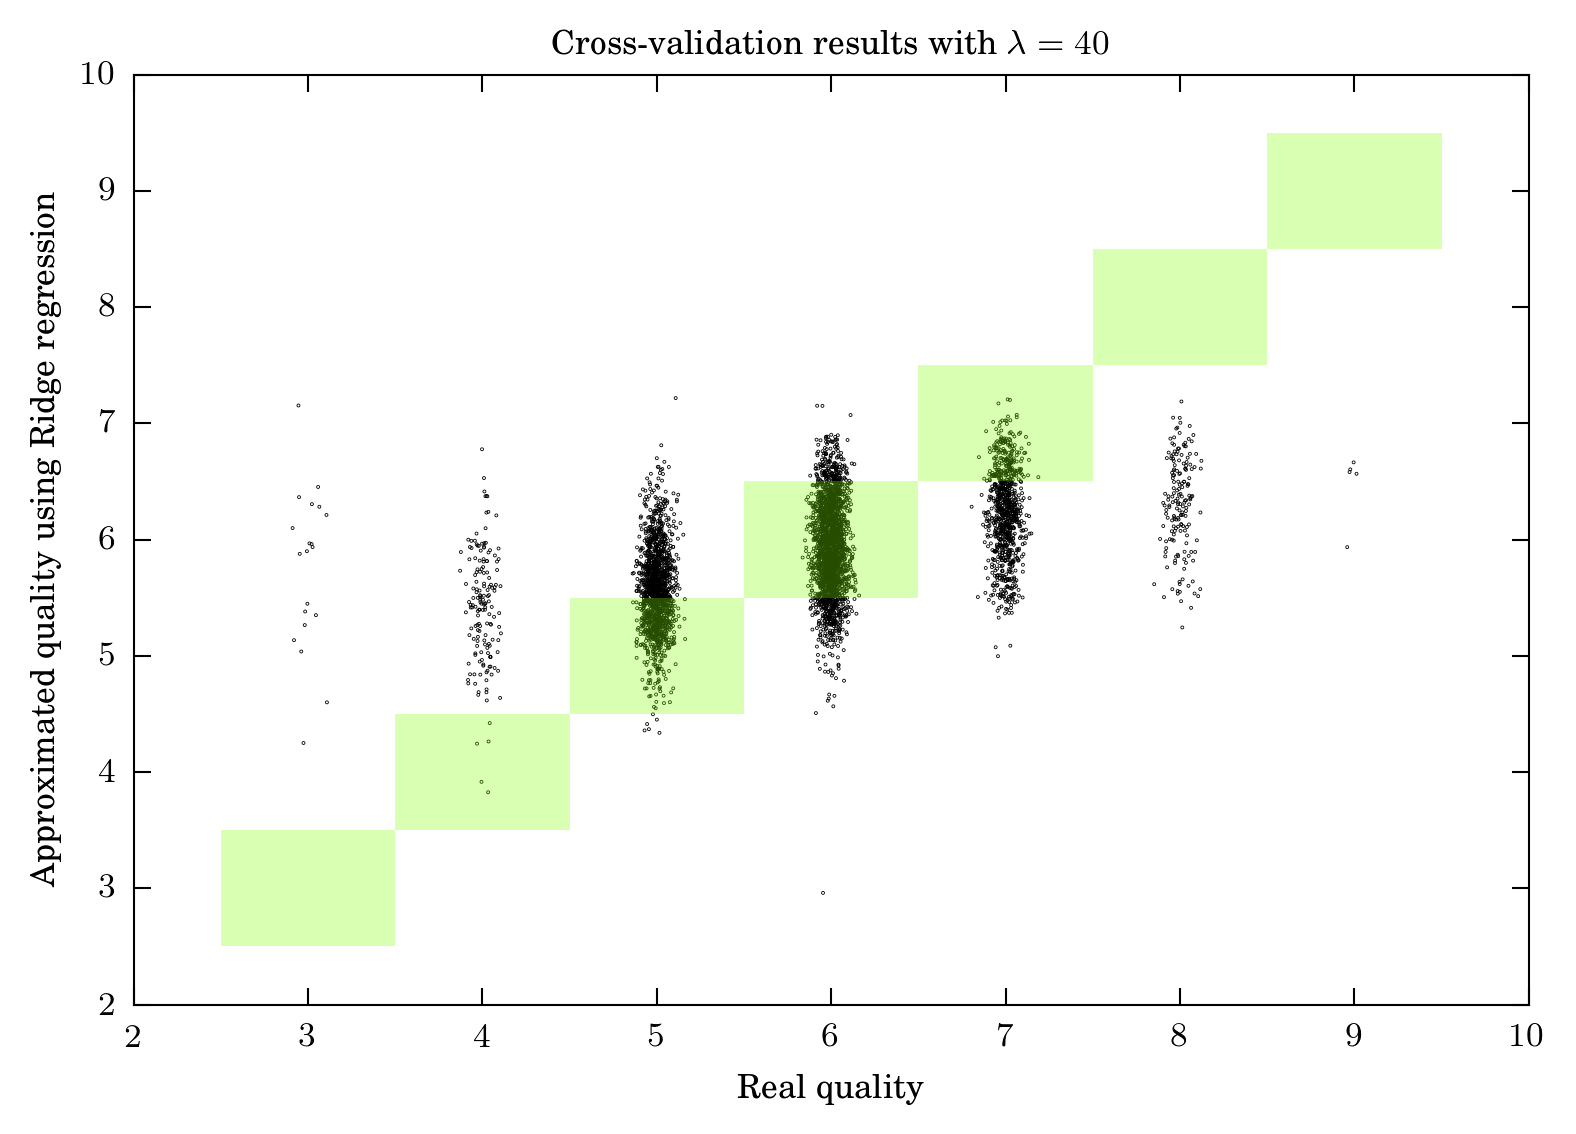
\includegraphics[width=\textwidth]{cv_scatters/reg_40.png}
\caption{Results of Ridge regression with $\lambda=40$}
\label{tbl:reg-scatter}
\end{figure}

\begin{figure}
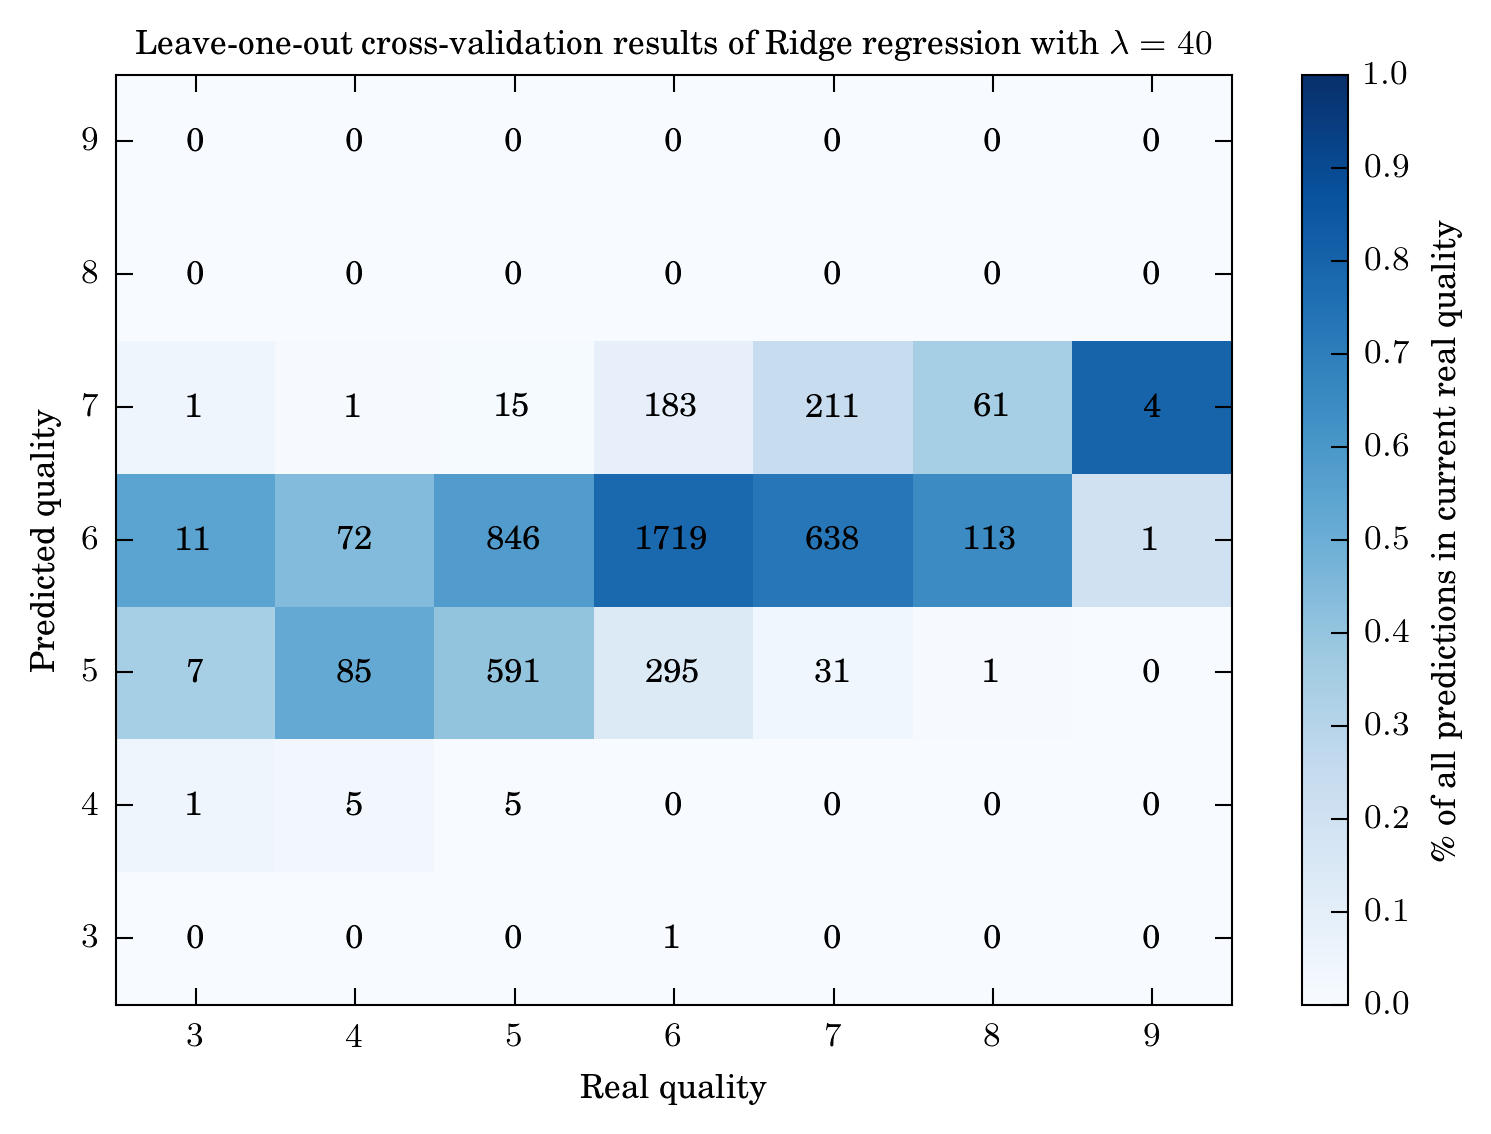
\includegraphics[width=\textwidth]{40-reg-heatmap.png}
\caption{Confusion matrix of Ridge regression cross-validation}
\label{tbl:reg-conf}
\end{figure}

\end{document}